%%%%%%%%%%%%%%%%%%%%%%%%%%%%%%%%%%%%%%%%%%%%%%%%%%%%%%%%%%%%%%%%%%%%%%%%%%%%%%%%%%%%%%%%%%%%%%%%%%%%%%
%
%   Filename    : chapter_3.tex 
%
%   Description : This file will contain your Research Methodology.
%                 
%%%%%%%%%%%%%%%%%%%%%%%%%%%%%%%%%%%%%%%%%%%%%%%%%%%%%%%%%%%%%%%%%%%%%%%%%%%%%%%%%%%%%%%%%%%%%%%%%%%%%%

\Section{Research Methodology}

This chapter discusses the systematic approach to be performed in order to accomplish the objectives of this research.

\subsection{Data Gathering}

During this stage, data gathering will be performed to identify the following: types of conceptual/semantic relations, appropriate semantic relations for the children's story domain, architecture of relation extraction systems and, algorithms for extracting conceptual relations. Additionally, the input corpus consisting of at least 30 children's stories will be gathered. Furthermore, interviews with English language professors and linguists will be conducted to verify the correctness of the input corpus. This means that if a corpus  contains dialogues, among other considerations, it is deemed incorrect. Thus, a modification of the corpus will be done to address the issue. If possible, manipulation of the input corpus will be done in order to fit the requirements of the tools to be utilized. The extraction templates will also be defined by analyzing the sentence structures in a children's story.  

There will be three types of modifications done on the corpus to remove dialogues. The first type of modification is done by transforming the dialogues into declarative sentences. The second type is the usual transformation of direct to indirect speech. And lastly, the third type of modification is the explicit addition of discourse markers whenever a dialogue is modified. After removing the dialogues, pronouns will also be removed and complex sentences will be simplified. Please see Appendix C for samples of each type of modification.

\subsection{Requirements Specification}

After gathering the data, the requirements will be defined and analyzed to determine the objectives and scope of the research. The resulting requirements specification will be validated to ensure completeness of the study and the tool to be developed. The final algorithm to be implemented should also be defined.

\begin{comment}
\begin{figure}[t]                %-- use [t] to place figure at top, [b] to place at the bottom
   \centering                    %-- use this to center the figure
   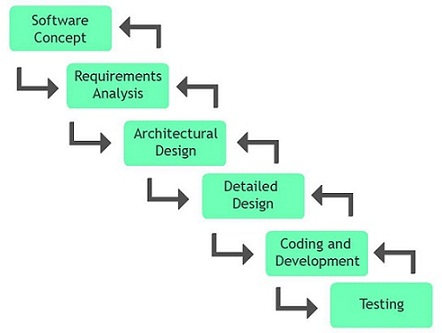
\includegraphics{methodology.jpg}      %-- include image file named as "sinag1.eps" 
   \caption{Modified Waterfall Model}
    \label{fig:methodology}
\end{figure}
\end{comment}

\subsection{Architectural Design}

In the Architectural Design stage, the different modules will be identified as well as the different external tools to be used. This includes a part-of-speech tagger, named-entity identifier, and text simplifier, among others. Other resources to be utilized will also be identified. Afterwards, the architectural design of the tool to be developed will be defined according to the final algorithm. Furthermore, the data structures which will represent the semantic relations in Picture Books will also be analyzed and designed. 

\begin{comment}
In the Architectural Design stage, the overall function and subsystems will be identified. Also, relationships, dependencies, and interactions among the subsystems will be determined. The resulting architectural design will be reviewed to help understand the flow and design of the system more.
\end{comment}

\subsection{Implementation}

The actual implementation of the architectural design as well as the final algorithm will be done in this stage. Debugging and unit testing will be done regularly to ensure the efficiency and correctness of the tool and algorithm.  

\subsection{Testing}

Testing will be done to ensure the quality and efficiency of the software. Unit testing for each subsystem will be performed. After doing so, integration testing will be performed to verify that each tool/subsystem receives the correct input from the previous tool/subsystem and generates the appropriate result for use by subsequent tools/subsystems. 

Test cases will be employed to check that all tools/subsystems interact correctly. System and functional testing will also be performed to check the functionality and performance of system functions. Lastly, the outputs of the system will mainly be evaluated through the use of Picture Books. The generated story of Picture Books after using the output semantic network will be evaluated by employing the same evaluation technique done in Picture Books. The output semantic network may also be evaluated by English language linguists to ensure the validity of the relations.

\subsection{Documentation}

Throughout the entire process of implementing the algorithm, documentation will be done to track its progress. This is also to ensure that any changes and implementations in the requirements of the study will be reflected in the documents.

\subsection{Calendar of Activities}

Tables \ref{tab:timetableactivities1} and \ref{tab:timetableactivities2} shows a Gantt chart of the activities. Each bullet represents approximately one week worth of activity. The overlapping activities ensure that any omissions and modifications will be changed immediately. 

%
%  the following commands will be used for filling up the bullets in the Gantt chart
%
\newcommand{\weekone}{\textbullet}
\newcommand{\weektwo}{\textbullet \textbullet}
\newcommand{\weekthree}{\textbullet \textbullet \textbullet}
\newcommand{\weekfour}{\textbullet \textbullet \textbullet \textbullet}

%
%  alternative to bullet is a star 
%
\begin{comment}
   \newcommand{\weekone}{$\star$}
   \newcommand{\weektwo}{$\star \star$}
   \newcommand{\weekthree}{$\star \star \star$}
   \newcommand{\weekfour}{$\star \star \star \star$ }
\end{comment}



\begin{table}[ht]   %t means place on top, replace with b if you want to place at the bottom
\centering
\caption{Timetable of Activities (Part 1)} \vspace{0.25em}
\begin{tabular}{|p{2in}|c|c|c|c|c|c|c|c|} \hline
\centering Activities (2010) & Jan & Feb & Mar & Apr & May & Jun & Jul \\ \hline
Data Gathering	       		& ~~~\weektwo & \weekfour & \weekfour & \weekfour &  &  &  \\ \hline
Requirements Specification	&  &  & ~~~\weektwo & \weekthree~~ &  &  &  \\ \hline
Architectural Design   		&  &  &  & ~~\weekthree & \weekfour & \weektwo~~~ &  \\ \hline
Implementation		   		&  &  &  &  & ~~~\weektwo & \weekfour & \weekfour  \\ \hline
Testing 			   		&  &  &  &  &  &  & \weekfour \\ \hline
Documentation 		   		& ~~~\weektwo & \weekfour & \weekfour & \weekfour & \weekfour & \weekfour & \weekfour \\ \hline
\end{tabular}
\label{tab:timetableactivities1}
\end{table}

\begin{table}[ht]   %t means place on top, replace with b if you want to place at the bottom
\centering
\caption{Timetable of Activities (Part 2)} \vspace{0.25em}
\begin{tabular}{|p{2in}|c|c|c|c|c|} \hline
\centering Activities (2010) & Aug & Sep & Oct & Nov & Dec \\ \hline
Data Gathering	       		 &  &  &  &  & \\ \hline
Requirements Specification   &  &  &  &  & \\ \hline
Architectural Design   		 &  &  &  &  & \\ \hline
Implementation		   		 & \weekfour & \weekfour &  &  & \\ \hline
Testing 			   		 & \weekfour & \weekfour & \weekfour & \weekfour & \\ \hline
Documentation 		   		 & \weekfour & \weekfour & \weekfour & \weekfour & \weekfour \\ \hline
\end{tabular}
\label{tab:timetableactivities2}
\end{table}




